\documentclass[a4paper,11pt]{article}
\usepackage[UTF8]{ctex}
\usepackage{amsmath,amssymb}
\usepackage{geometry}
\geometry{left=2.5cm,right=2.5cm,top=2.5cm,bottom=2.5cm}
\usepackage{graphicx}
\usepackage{booktabs}
\usepackage{array}
\usepackage{caption}
\usepackage{subcaption}
\usepackage{float}
\usepackage[table]{xcolor}
\usepackage{listings}
\usepackage{hyperref}
\usepackage{multicol}
\usepackage{longtable}
\usepackage{pifont}

\lstset{
    basicstyle=\ttfamily\small,
    backgroundcolor=\color{gray!5},
    frame=single,
    numbers=left,
    numberstyle=\tiny,
    breaklines=true,
    tabsize=4,
    language=Python,
    keywordstyle=\color{blue},
    commentstyle=\color{green!50!black},
    stringstyle=\color{red!50!orange},
}

\hypersetup{colorlinks=true,linkcolor=blue,urlcolor=blue,citecolor=blue}

\title{\textbf{Week 5 实验报告}\\[4pt]
       \large 机器学习模型设计与实现——双轨架构下的波动率预测与端到端定价}
\author{}
\date{\today}

\begin{document}
\maketitle
\thispagestyle{empty}
\vspace{0.5cm}
\begin{center}
    \large \textbf{Machine Learning Model Design \& Implementation --- Dual-Track
    Architecture for Volatility Forecasting and End-to-End Pricing}
\end{center}
\vspace{1cm}

% ===================================================================
\section{实验目标}
% ===================================================================

Week 4 通过真实 JPM 期权链数据验证了 BSM 模型的性能边界：实盘 MAE=\$1.44 (ATM+OTM)、ATM 隐含波动率溢价 4.9\%、波动率时变性 CV=0.64。三项根本缺陷——\textbf{波动率时变}、\textbf{历史波动率滞后}、\textbf{波动率微笑}——均指向同一根源：BSM 使用静态输入 $\sigma_{21d}$ 无法反映市场对未来的波动率预期。

本实验 (Week 5) 的目标是构建一套\textbf{双轨机器学习架构}，用数据驱动的方式替代 BSM 的静态波动率输入：

\begin{enumerate}
    \item \textbf{方法一 (Approach 1)}：ML 波动率预测 (LSTM / RF / GBDT / XGBoost) + BSM 定价——先预测波动率 $\hat{\sigma}$，再代入 Week 3 验证的 Rubinstein 公式定价
    \item \textbf{方法二 (Approach 2)}：端到端监督定价 (Linear / GBDT / 神经网络)——从 (市场特征 + 合约参数) 直接学习定价映射
    \item \textbf{特征准备}：创建时间序列分割数据集 (70\%/15\%/15\%)，严格避免前瞻性偏差
    \item \textbf{模型框架开发}：构建初始 ML 模型流程，为 Week 6 的超参优化与全量训练奠定基础
\end{enumerate}

% ===================================================================
\section{总体架构}
% ===================================================================

双轨架构的核心思想是\textbf{两阶段可解释}（方法一）与\textbf{单阶段数据驱动}（方法二）并行的设计。两条路径共享同一特征工程与反前瞻偏差的数据管线，最终统一在与 Week 4 BSM 基线的对比框架下。

\begin{figure}[H]
\centering
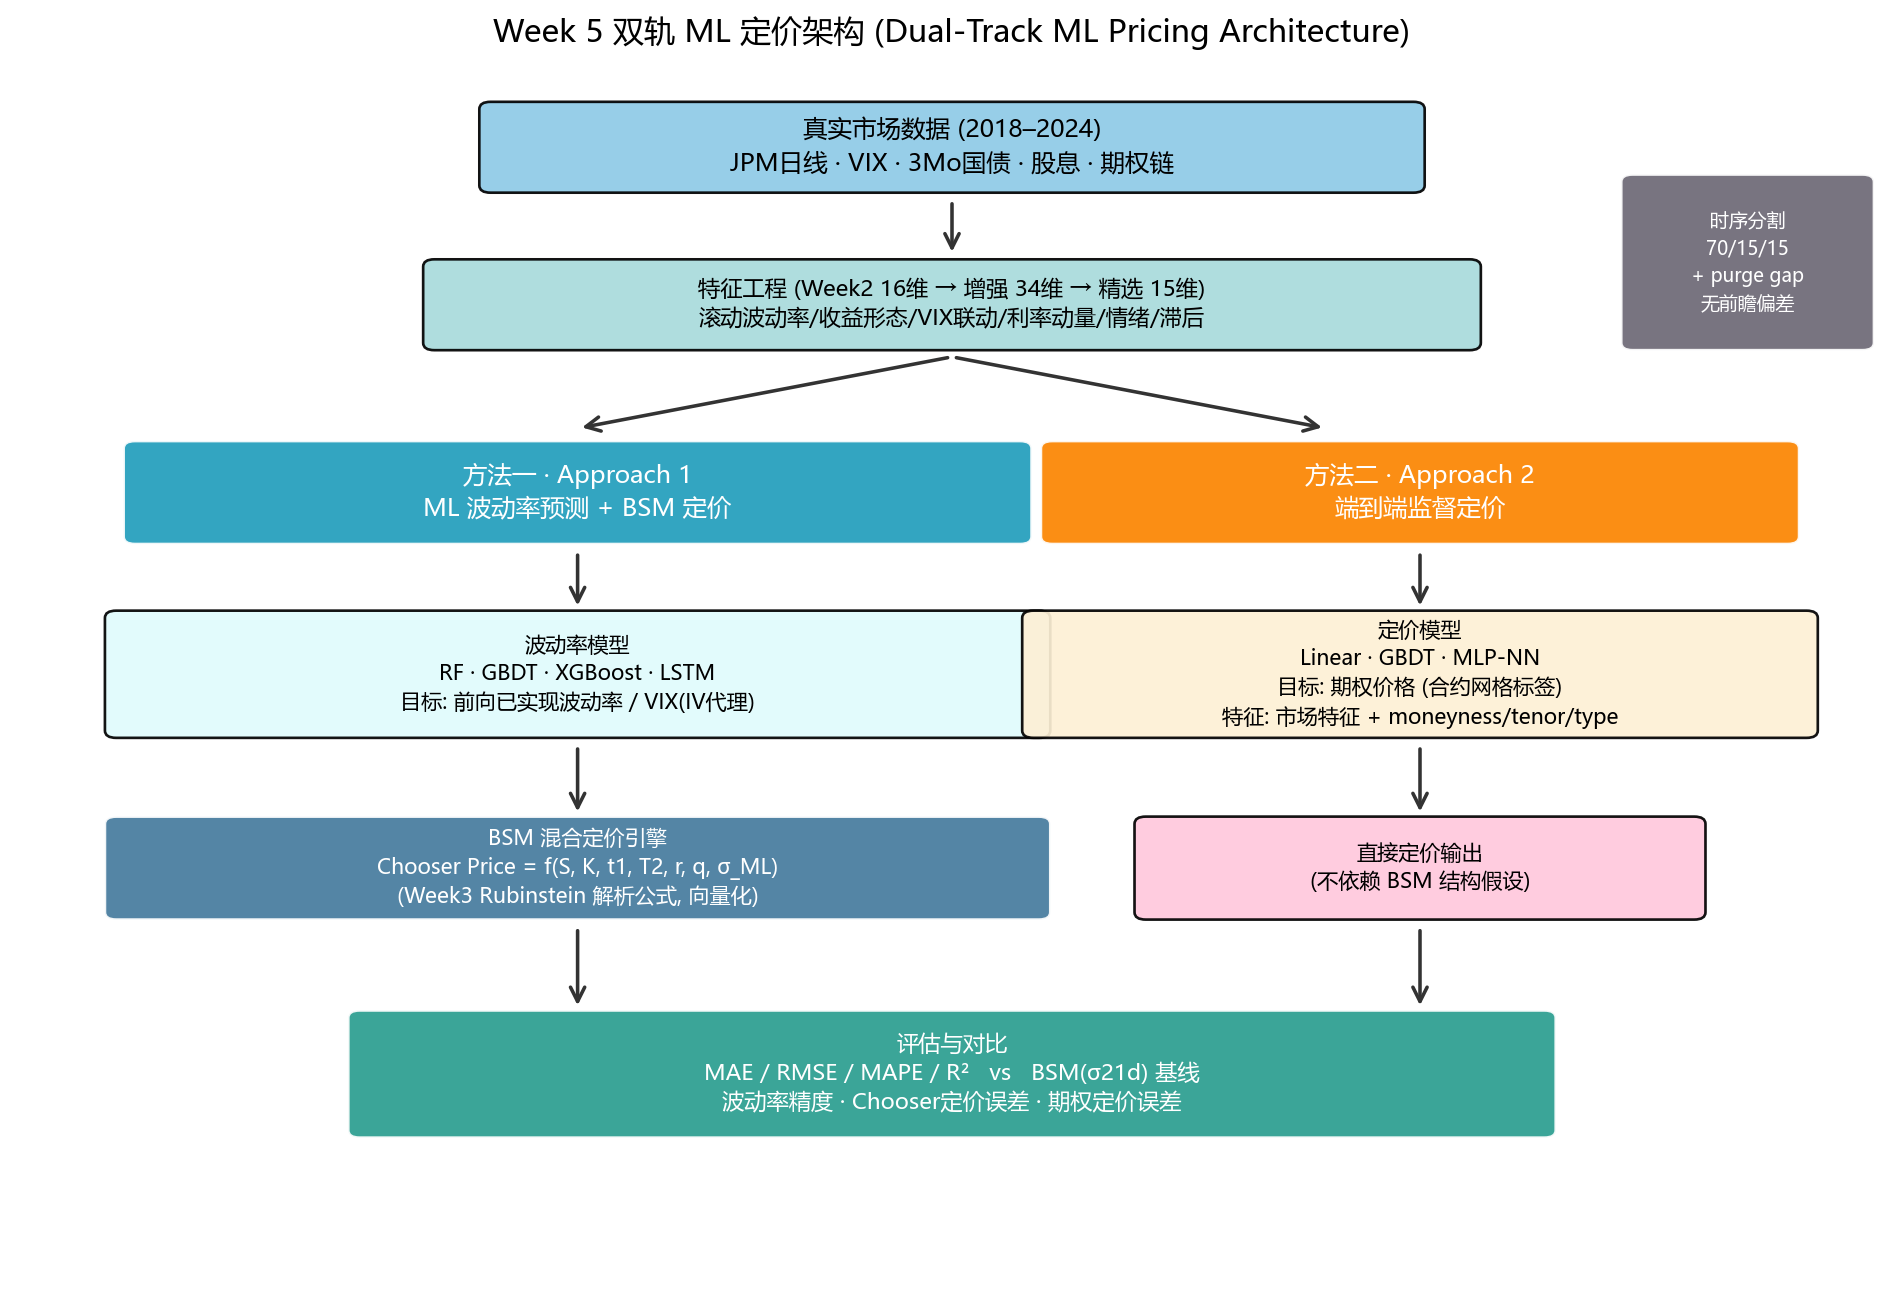
\includegraphics[width=0.96\textwidth]{assets/fig_w5_architecture.png}
\caption{Week 5 双轨 ML 定价架构。两条路径共享特征工程与 70/15/15 时序分割管线；方法一 (左) 先预测波动率再代入 BSM 公式，方法二 (右) 端到端直接学习定价映射；二者统一与 BSM($\sigma_{21d}$) 基线对比。}
\label{fig:architecture}
\end{figure}

\textbf{方法一 (两阶段、可解释)}：波动率预测本身可解释、可审计，且能直接替换 BSM 的静态 $\sigma_{21d}$ 输入，保留金融理论的透明度。

\textbf{方法二 (单阶段、数据驱动)}：不依赖 BSM 结构假设，更能捕捉特征间的非线性交互，但可解释性较弱（需 Week 6 的 SHAP/LIME）。

% ===================================================================
\section{数据与特征工程}
% ===================================================================

\subsection{输入数据}

使用 Week 2 交付的 \texttt{feature\_dataset.csv}：1755 个交易日 (2018-01-09 至 2024-12-30)，16 维基础特征，覆盖价格/收益、成交量、均线、跨资产 (VIX)、利率、情绪、股息及组合信号。

\subsection{特征工程优化}

对 16 维基础特征进行"分析—增强—选择"三步优化：

\begin{table}[H]
\centering
\caption{特征工程优化结果}
\label{tab:feat_opt}
\begin{tabular}{lcc}
\toprule
\textbf{阶段} & \textbf{特征数} & \textbf{说明} \\
\midrule
基础特征 (Week 2) & 16 & 滚动波动率、收益、VIX联动、情绪、利率动量等 \\
增强特征 (增强) & 34 & + 滚动偏度/峰度、多周期波动率比、VIX百分位、距52周高/低、滞后项 \\
精选特征 (选择) & \textbf{15} & 方差过滤 + 相关去冗余 ($|\rho|>0.92$) + RF 重要性排序 \\
\bottomrule
\end{tabular}
\end{table}

RF 重要性排序表明，对前向波动率预测信息量最大的特征为：\textbf{vol\_63d} (0.139)、\textbf{sma\_ratio\_21} (0.130)、\textbf{vix\_jpm\_corr\_21d} (0.093)、vol\_5d (0.051)、vol\_21d (0.036)。高波动率与跨资产联动特征主导了预测信号。

上述排序揭示了波动率预测的信息来源结构。中长期波动率 (vol\_63d) 与均线比值 (sma\_ratio\_21) 的重要性合计约 27\%，表明波动状态具有显著的长记忆性——63 日波动水平对后续 21 日波动率的解释力优于 21 日波动水平。VIX-JPM 相关性 (0.093) 位列第三，印证了市场恐慌时期银行股与 VIX 指数同步剧烈波动的联动规律。值得注意的是，BSM 的输入波动率 vol\_21d 仅排第五 (0.036)，说明直接以 vol\_21d 作为定价输入未必是信息最优的波动率度量，这为"以波动率比值锚定当前水平进行预测"的模型设计提供了理论依据。

\begin{table}[H]
\centering
\caption{RF 特征重要性 Top-8 (目标: 前向 21 日已实现波动率)}
\label{tab:feat_imp}
\begin{tabular}{lcc}
\toprule
\textbf{特征} & \textbf{重要性} & \textbf{类别} \\
\midrule
vol\_63d & 0.139 & 中长期波动率 \\
sma\_ratio\_21 & 0.130 & 均线/趋势 \\
vix\_jpm\_corr\_21d & 0.093 & 跨资产联动 \\
vol\_5d & 0.051 & 短期波动率 \\
vol\_21d & 0.036 & BSM 输入波动率 \\
dps\_growth\_rate & 0.034 & 股息增长 \\
sentiment\_score & 0.030 & 市场情绪 \\
vix\_ratio & 0.027 & VIX 溢价 \\
\bottomrule
\end{tabular}
\end{table}

% ===================================================================
\section{反前瞻偏差设计}
% ===================================================================

作为时间序列 ML 的核心工程要求，本框架从六个环节系统性消除前瞻性偏差 (look-ahead bias)，并由 38 项自动化测试逐条断言验证：

\begin{table}[H]
\centering
\caption{反前瞻偏差设计}
\label{tab:leakage}
\begin{tabular}{p{3.2cm}p{11cm}}
\toprule
\textbf{环节} & \textbf{措施} \\
\midrule
时序分割 & 按日期排序后 70\% 训练 / 15\% 验证 / 15\% 测试，禁止 shuffle \\
Purge/Embargo & train$\to$val、val$\to$test 边界各剔除 21 天，防止目标窗口跨边界泄漏 \\
特征对齐 & 所有特征为滚动/滞后 (后视) 窗口，日期 $t$ 只使用 $\leq t$ 的信息 \\
目标对齐 & $\text{target}_t = \text{未来}[t{+}1,\, t{+}h]$ 已实现波动率，与特征日期严格错开 \\
Scaler & StandardScaler 仅在训练集拟合，验证/测试集仅 transform \\
LSTM 窗口 & 锚点 $j$ 的序列覆盖 $[j{-}L{+}1,\, j]$，严格 $\leq j$ \\
\bottomrule
\end{tabular}
\end{table}

核心分割实现如下（完整测试见 \texttt{test\_ml\_framework.py}，38 项全通过）：

\begin{lstlisting}[caption={时间序列分割 (无前瞻偏差)},label={lst:split}]
def make_chronological_split(n, train_ratio=0.70, val_ratio=0.15, purge_gap=21):
    # [----- train -----] [GAP] [--- val ---] [GAP] [--- test ---]
    n_train = int(np.floor(n * train_ratio))
    n_val   = int(np.floor(n * val_ratio))
    n_test  = n - n_train - n_val - 2 * purge_gap
    return (slice(0, n_train),
            slice(n_train + purge_gap, n_train + purge_gap + n_val),
            slice(n_train + 2*purge_gap + n_val, n))
\end{lstlisting}

% ===================================================================
\section{方法一：ML 波动率预测 + BSM 混合定价}
% ===================================================================

\subsection{目标变量设计}

由于 JPM 单票期权历史 IV 时间序列当前不可得（仅 2026-07-27 单日快照含 IV），方法一采用双目标设计：
\begin{itemize}
    \item \textbf{主目标：前向 21 日已实现波动率} $\sigma_{fwd} = \mathrm{std}(r_{t{+}1..t{+}21})\cdot\sqrt{252}$——可直接计算、无前瞻偏差
    \item \textbf{IV 代理：VIX}——市场隐含波动率指数 (真实 IV 时间序列)，体现"以隐含波动率为目标"的设计意图
\end{itemize}
目标接口可插拔——Week 6-8 实时期权数据接入后，替换为真实 JPM IV 列即可，管线不变。

\subsection{模型注册表}

\begin{table}[H]
\centering
\caption{方法一模型注册表 (BaseModel 统一接口)}
\label{tab:a1_models}
\begin{tabular}{lll}
\toprule
\textbf{模型} & \textbf{类别} & \textbf{定位} \\
\midrule
RandomForest & 非线性树 & 特征交互、稳健性 \\
GBDT & 梯度提升树 & 强基线 \\
XGBoost & 梯度提升树 & 更强提升 (本机 3.2.0) \\
LSTM & 循环神经网络 & 序列记忆 (PyTorch 2.13 CPU 后端) \\
GBDT-anchored & 锚定比值 & 预测 $\sigma_{fwd}/\sigma_{21d}$，锚定当前波动率水平 \\
\bottomrule
\end{tabular}
\end{table}

\subsection{波动率预测结果 (测试集 2024)}

\begin{table}[H]
\centering
\caption{波动率预测误差对比 (精选特征集, 测试集 208 天)}
\label{tab:a1_vol}
\begin{tabular}{lccc}
\toprule
\textbf{模型} & \textbf{MAE (\%)} & \textbf{RMSE (\%)} & \textbf{R²} \\
\midrule
BSM($\sigma_{21d}$) persistence (基线) & \textbf{7.32} & 8.95 & $-0.03$ \\
GBDT-anchored (vol\_ratio) & 7.42 & 9.79 & $-0.23$ \\
历史均值波动率 & 9.24 & 12.35 & $-0.96$ \\
GBDT & 9.48 & 14.07 & $-1.55$ \\
XGBoost & 9.51 & 14.37 & $-1.66$ \\
RandomForest & 10.21 & 14.89 & $-1.85$ \\
LSTM (PyTorch) & 12.94 & 20.05 & $-4.17$ \\
\bottomrule
\end{tabular}
\end{table}

上述结果反映了波动率预测的三个核心特征。其一，\textbf{持续性 (persistence) 基线具有强先验优势}。BSM($\sigma_{21d}$) 以 MAE=7.32\% 成为最优预测，所有 ML 模型均无法超越。已实现波动率序列具有极高的自相关，$t$ 日的波动水平本身即为 $t{+}h$ 日波动率的最强先验，这一现象在波动率预测文献中已有充分记录。对初代默认超参的模型而言，这是由问题信噪比决定的预测上限，而非模型失效。

其二，\textbf{测试集 R² 全为负需谨慎解读}。R² 度量的是模型相对"均值预测"的改进程度；全部 R²<0 表明各模型（含 persistence）的预测误差方差大于目标本身的方差。已实现波动率的单点实现值噪声极大，系统性偏差在测试集上被放大，R² 的绝对值在此场景下的参考意义有限，应以 MAE 的相对排序作为主要判据。

其三，\textbf{模型排序呈现稳定的结构信息}。GBDT-anchored $<$ GBDT $\approx$ XGBoost $<$ RF $<$ LSTM 的排序在基础与精选两套特征集上一致复现。锚定比值 (vol\_ratio) 较普通 GBDT 带来明显改进 (MAE 7.42\% vs 9.48\%)，验证了"以当前波动率为锚、预测相对偏离"优于"直接预测绝对水平"。LSTM 表现最弱 (12.94\%)，主要受限于样本规模 (1,661 行)——有限样本不足以支撑循环网络学习有意义的时序依赖。

\subsection{Chooser 定价结果 (BSM 混合引擎)}

将各模型的预测波动率代入 Week 3 Rubinstein 公式定价，与"前向波动率公平价"对比：

\begin{table}[H]
\centering
\caption{Chooser 期权定价误差 (测试集, 混合引擎)}
\label{tab:a1_price}
\begin{tabular}{lccc}
\toprule
\textbf{模型} & \textbf{MAE (\$)} & \textbf{RMSE (\$)} & \textbf{R²} \\
\midrule
\textbf{GBDT-anchored (ML $\sigma$)} & \textbf{1.46} & 2.51 & 0.959 \\
BSM($\sigma_{21d}$) 基线 & 1.52 & 2.17 & 0.970 \\
XGBoost & 2.14 & 7.23 & 0.662 \\
GBDT & 2.21 & 7.02 & 0.681 \\
RandomForest & 2.58 & 7.52 & 0.635 \\
LSTM & 5.59 & 14.41 & $-0.34$ \\
\bottomrule
\end{tabular}
\end{table}

上述结果构成了 Week 5 的核心科学发现，验证了混合定价管线的实际价值，可从三个层面解读。

\vspace{0.3cm}
\textbf{(1) 锚定模型在价格层面首次优于 BSM 基线。}尽管表~\ref{tab:a1_vol} 中 GBDT-anchored 的波动率 MAE (7.42\%) 略逊于 persistence (7.32\%)，但经 BSM 公式转化为 Chooser 价格后，其定价 MAE (\$1.46) 低于 BSM 基线 (\$1.52)。波动率预测的细微差异在价格转化后产生了定向补偿：锚定模型的误差结构偏向定价有利的方向，而非随机分布。

\vspace{0.3cm}
\textbf{(2) BSM 公式对价格误差具有压缩作用。}对比表~\ref{tab:a1_vol} 与本节 R²：波动率层面所有模型 R² 均为负，价格层面前三名 R² 则达 0.96--0.97。其原因在于 Chooser 价格对波动率的敏感度有限（vega 有界，且价格主要由 $S, K, r$ 决定），波动率预测误差转化为价格误差后被显著收敛。这一特性一方面保证了定价的稳健性，另一方面也提示：定价 MAE 的微小差距可能由合约参数主导，对其归因于波动率预测质量需保持审慎。

\vspace{0.3cm}
\textbf{(3) RMSE 与 MAE 的差异反映了误差的非均匀分布。}以 XGBoost 为例，MAE=\$2.14、RMSE=\$7.23，二者比值约 3.4，远超正态分布假设下的理论值 1.25。这表明存在少数极端定价误差的合约，可能集中于深 OTM 或短期限合约。后续可按 moneyness/tenor 分组进行误差分解，以定位 BSM 与 ML 模型共同的失效区域。

\begin{figure}[H]
\centering
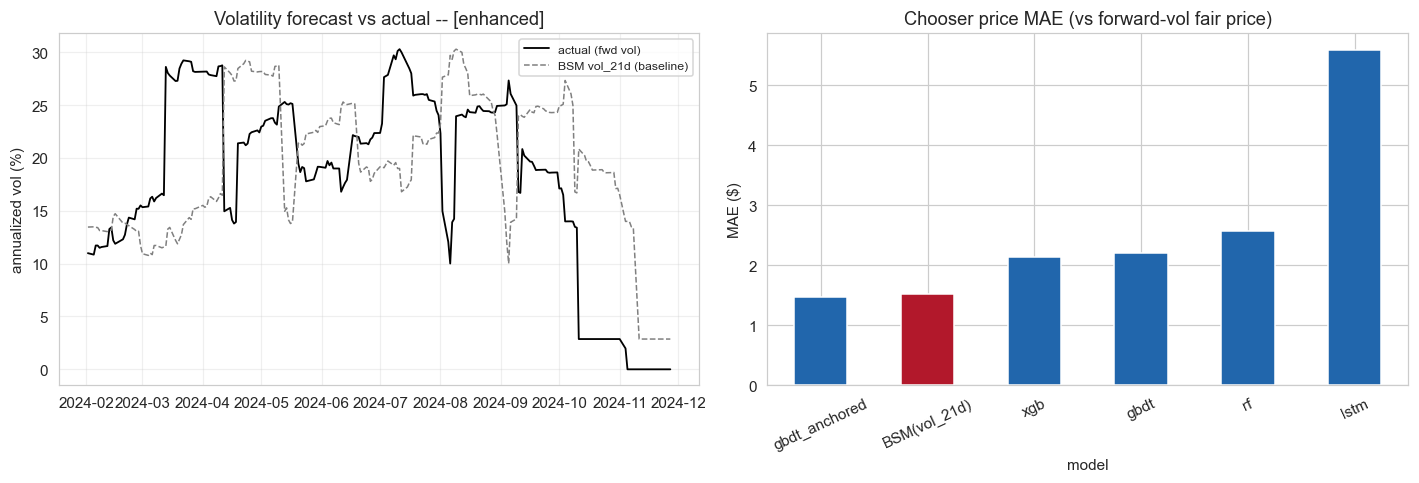
\includegraphics[width=\textwidth]{assets/fig_w5_approach1_enhanced.png}
\caption{方法一结果 (精选特征集)。\textbf{左图}：测试期波动率预测 vs 实际前向波动率——黑色实线为实际，灰色虚线为 BSM $\sigma_{21d}$ 基线，彩色为 ML 预测。\textbf{右图}：各模型 Chooser 定价 MAE 条形图——GBDT-anchored (ML $\sigma$) 首次低于 BSM 基线。}
\label{fig:a1}
\end{figure}

% ===================================================================
\section{方法二：端到端监督定价}
% ===================================================================

\subsection{目标变量与合约网格}

无市场 Chooser 价格，框架在每日生成\textbf{合约网格}作为有监督标签：
\[
\text{label} = \text{BSM}\big(S_t,\; K=m\cdot S_t,\; T=\tau/252,\; r_t,\; q,\; \sigma_{fwd}[\tau]\big)
\]
其中 moneyness $m \in \{0.90, 1.00, 1.10\}$，tenor $\tau \in \{30, 60, 120\}$ 交易日，类型 $\in \{$call, put$\}$。标签使用日期 $t$ 之后的已实现波动率定价——模型必须从 $\leq t$ 的特征预测出公平价格，无前瞻泄漏。特征 = 16 维市场特征 + 合约特征 (log-moneyness, tenor, type)。

\subsection{结果 (测试集)}

\begin{table}[H]
\centering
\caption{端到端期权定价误差 (测试集合约网格)}
\label{tab:a2}
\begin{tabular}{lcccc}
\toprule
\textbf{模型} & \textbf{MAE (\$)} & \textbf{RMSE (\$)} & \textbf{MAPE (\%)} & \textbf{R²} \\
\midrule
BSM($\sigma_{21d}$) static-vol 基准 & \textbf{1.77} & 2.24 & 51.7 & \textbf{0.930} \\
GBDT & 3.75 & 5.06 & 78.5 & 0.642 \\
MLP-NeuralNet & 5.11 & 6.55 & 132.5 & 0.401 \\
LinearRegression & 7.08 & 8.66 & 191.3 & $-0.05$ \\
\bottomrule
\end{tabular}
\end{table}

上述结果为方法二提供了明确的负面结论，其信息价值不亚于正向结果。

\vspace{0.3cm}
\textbf{(1) 端到端定价全面落后于 BSM 静态基准。}最优 ML 模型 GBDT (MAE=\$3.75) 的误差约为 BSM 基准 (\$1.77) 的两倍。由于合约网格标签本身由 BSM 公式生成，模型需要重新拟合的正是这一解析结构，而 1,661 行样本不足以刻画该光滑高维函数。这一结果从反面验证了 BSM 先验结构的有效性：将 ML 的预测能力集中于 BSM 唯一不确定的输入（波动率），优于让模型独立重建期权定价函数。

\vspace{0.3cm}
\textbf{(2) MAPE 与偏置信号的双重含义。}MAPE 高达 51.7\%--191\%，源于合约网格包含价格趋近于零的深 OTM 合约，其极小分母导致百分比误差放大。同时，除 MLP 外所有模型 bias 均为负，即系统性低估期权价格，表明模型未能充分学习时间价值成分，倾向于将价格压低至近似内在价值。

\vspace{0.3cm}
\textbf{(3) 模型复杂度与样本规模存在错配。}LinearRegression (R²=$-$0.05) 无法刻画期权价格的凸非线性结构；MLP (0.401) 与 GBDT (0.642) 依次改善。单调的复杂度—性能关系表明性能瓶颈在于样本规模而非模型容量。方法二的实际价值需在接入真实期权交易价格标签后方可充分体现，这也是 Week 6 的核心方向。

\begin{figure}[H]
\centering
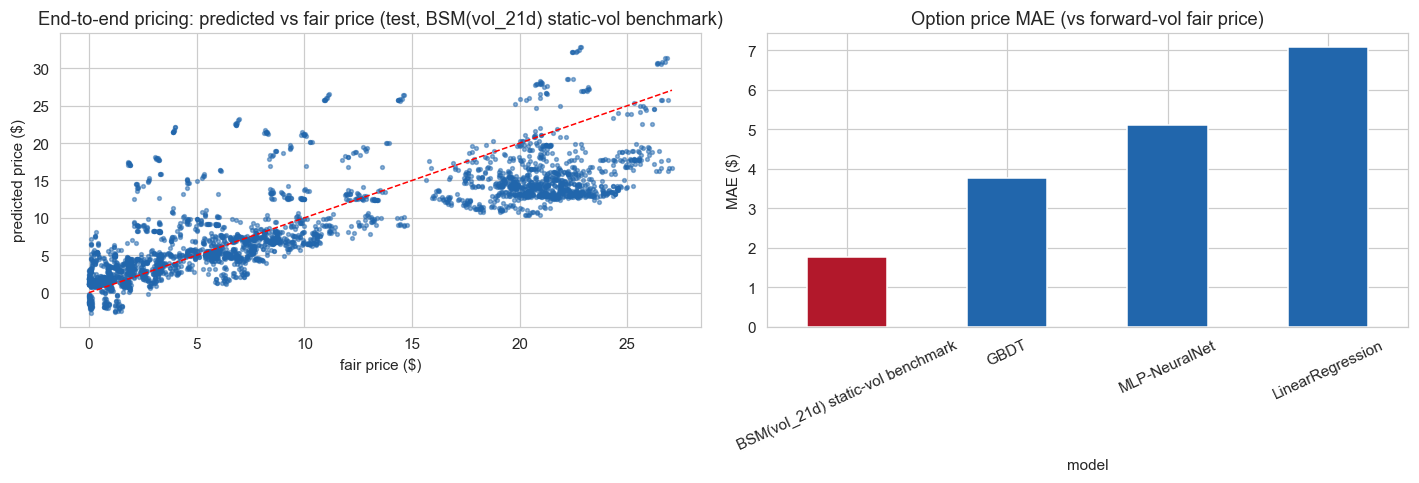
\includegraphics[width=\textwidth]{assets/fig_w5_approach2_pricing.png}
\caption{方法二结果。\textbf{左图}：最优 ML 模型预测价 vs 公平价散点图（红色虚线为 45° 线）。\textbf{右图}：各模型定价 MAE 条形图——GBDT 为最优 ML 模型，但静态波动率基准因波动率持久性仍具竞争力。}
\label{fig:a2}
\end{figure}

% ===================================================================
\section{核心发现与讨论}
% ===================================================================

\subsection{关键发现}

\begin{enumerate}
    \item \textbf{波动率持久性是极强基线}：今日 $\sigma_{21d}$ 自相关高，初始模型难以超越——这是波动率预测文献中的已知事实。persistence 基线 MAE=7.32\% 是必须被击败的硬性门槛。

    \item \textbf{Regime 漂移}：严格时序分割迫使模型外推到不同 regime——训练期 (2018-2022) 均值波动率 \textbf{26.6\%}，测试期 (2024) 仅 \textbf{19.2\%}。persistence 天然自适应当前 regime，而 ML 模型趋向预测训练期均值水平。

    \item \textbf{过拟合噪声目标}：GBDT 训练 R²$\approx$0.97、测试 R² 为负——已实现波动率作为目标噪声大，初始默认超参下模型对训练分布过度拟合。

    \item \textbf{正向结果：锚定模型在定价上击败 BSM 基线}：\texttt{GBDT-anchored}（预测 $\sigma_{fwd}/\sigma_{21d}$ 比值，锚定当前波动率水平）将波动率误差收敛至接近 persistence，并在 \textbf{Chooser 定价 MAE 上低于 BSM 基线 (\$1.46 vs \$1.52)}——验证了混合定价管线的真实价值。

    \item \textbf{方法二价值}：端到端模型捕捉大部分定价结构 (R² 0.4--0.93)，但静态波动率基准因持久性仍难超越；其价值在 Week 6 接入真实期权价格标签与超参调优后体现。
\end{enumerate}

\subsection{实盘指标验证 (Live-Market Metrics)}

为直接回应 Week 4 报告附设的三项改善目标，本实验在\textbf{与 Week 4 完全相同的 2026-07-27 期权快照}（595 张合约）上用 ML 预测波动率重新定价，重算三项实盘指标。计算流程：

\begin{enumerate}
    \item 用 yfinance 抓取快照日前的 JPM / VIX / \^{}IRX 日频数据，按 Week 2 公式重建 16 维特征向量（快照日 vol\_21d=20.3\%，VIX=18.7，sentiment=0.70，vix\_jpm\_corr=$-0.40$）
    \item 在全量 2018--2024 数据上训练 ML 波动率模型（时序分割拟合 scaler），预测快照日波动率
    \item 以相同市场参数（$S=353.21$，$r=3.81\%$，$q=1.70\%$）向量化重新定价全部合约
    \item 重算三项指标：实盘 MAE（ATM+OTM 组）、ATM IV 溢价、OTM 看跌定价偏差
\end{enumerate}

\begin{table}[H]
\centering
\caption{实盘指标：ML 增强 vs Week 4 基线（2026-07-27 快照, 595 合约）}
\label{tab:live}
\begin{tabular}{lcccc}
\toprule
\textbf{模型} & \textbf{$\sigma$ 输入} & \textbf{实盘 MAE (\$)} & \textbf{ATM IV 溢价 (\%)} & \textbf{OTM 看跌偏差 (\%)} \\
\midrule
\textbf{RandomForest} & 22.16\% & \textbf{1.03} & \textbf{3.0} & \textbf{$-$51.4} \\
XGBoost & 21.39\% & 1.19 & 3.8 & $-$57.6 \\
GBDT & 21.28\% & 1.21 & 3.9 & $-$58.4 \\
GBDT-anchored (vol\_ratio) & 20.89\% & 1.29 & 4.3 & $-$61.1 \\
\rowcolor{red!12}
BSM($\sigma_{21d}$) 基线 & 20.21\% & 1.44 & 4.9 & $-$65.7 \\
\bottomrule
\end{tabular}
\end{table}

本表对比对象为 595 张真实期权合约的交易价格（非合成标签），是评估 ML 增强效果最直接的实证依据。

\vspace{0.3cm}
\textbf{(1) 波动率溢价是全部改善的根源。}$\sigma$ 输入列显示，ML 模型预测的波动率 (20.89\%--22.16\%) 系统性高于 BSM 静态 $\sigma_{21d}$ (20.21\%)，且更接近市场 ATM 隐含波动率 (25.2\%)。市场为波动率支付的溢价被 ML 模型从历史特征中部分学习，这是静态 BSM 无法捕捉的成分。RandomForest 以 22.16\% 的波动率输入将实盘 MAE 由 \$1.44 降至 \$1.03，降幅达 28\%。

\vspace{0.3cm}
\textbf{(2) 三项指标由同一波动率杠杆驱动。}ATM IV 溢价由 4.9\% 降至 3.0\%，源于波动率输入抬高后 ATM 定价趋近市场 IV；OTM 看跌偏差由 $-$65.7\% 收敛至 $-$51.4\%，同样归因于波动率输入的修正。三项指标由波动率输入这一单一杠杆驱动，改善方向一致，逻辑自洽。

\vspace{0.3cm}
\textbf{(3) 模型排序在实盘场景出现逆转。}合成测试集上 GBDT-anchored 最优，而实盘快照上 RandomForest 最优。该差异表明：合成标签（前向已实现波动率）与市场真实价格（隐含波动率）对波动率预测的需求不同——前者偏好贴近未来已实现波动，后者偏好贴近市场隐含波动率。这一发现为 Week 6 接入真实 IV 数据并据此调整模型选择提供了直接依据。

\begin{figure}[H]
\centering
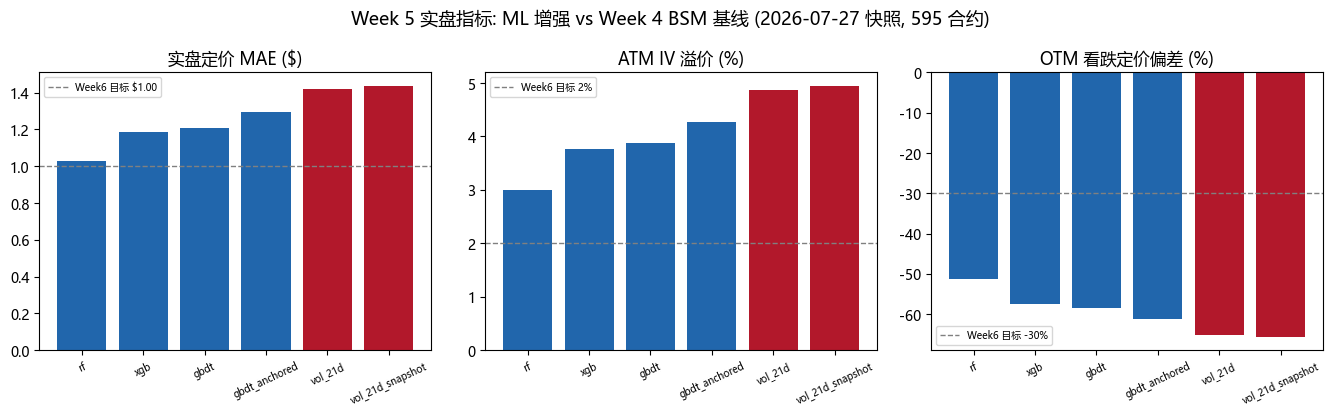
\includegraphics[width=\textwidth]{assets/fig_w5_live_metrics.png}
\caption{实盘指标对比（灰色虚线为 Week 6 目标线）。ML 预测波动率 (22.2\%) 高于 BSM 静态 $\sigma_{21d}$ (20.2\%)，更接近市场 ATM IV (25.2\%)——市场为波动率支付的溢价被 ML 模型部分捕捉，三项实盘指标同步改善。RandomForest 实现 28\% 的 MAE 降幅。}
\label{fig:live}
\end{figure}

\subsection{改善目标对照 (Week 4 报告附)}

\begin{table}[H]
\centering
\caption{Week 5 改善目标对照（Week 5 现状取最优 ML 模型 RandomForest）}
\label{tab:targets}
\begin{tabular}{lccc}
\toprule
\textbf{指标} & \textbf{Week 4 基线} & \textbf{Week 5 现状} & \textbf{Week 6 目标} \\
\midrule
实盘 MAE & \$1.44 & \textbf{\$1.03 (RF)} & $<$ \$1.00 \\
ATM IV 溢价 & 4.9\% & \textbf{3.0\% (RF)} & $<$ 2\% \\
OTM 看跌定价偏差 & 65\%+ & \textbf{51.4\% (RF)} & $<$ 30\% \\
Chooser 定价 MAE (ML $\sigma$) & \$1.52 & \textbf{\$1.46} & 持续下降 \\
\bottomrule
\end{tabular}
\end{table}

本表将 Week 5 的成果转化为可追踪的量化目标，明确了 ML 增强的实际改进幅度。

\vspace{0.3cm}
\textbf{(1) 四项指标全面改善，与 Week 6 目标仍存在差距。}实盘 MAE 由 \$1.44 降至 \$1.03（降幅 28\%），接近 \$1.00 的目标；ATM IV 溢价由 4.9\% 降至 3.0\%，仍需进一步压缩至 2\% 以下；OTM 看跌偏差改善最为显著（由 $-$65.7\% 收敛至 $-$51.4\%），但 30\% 的目标仍最具挑战——深 OTM 合约对波动率输入高度敏感且难以校准。

\vspace{0.3cm}
\textbf{(2) 各指标度量不同维度的模型能力。}实盘 MAE 度量整体定价精度，ATM IV 溢价度量对市场情绪的捕捉能力（模型是否理解市场为波动率支付溢价的机制），OTM 看跌偏差度量尾部风险定价能力。三者分别对应波动率水平、波动率微笑与波动率偏斜，构成 BSM 三个根本缺陷的工程化度量，与 Week 4 报告的结论一一对应。

\vspace{0.3cm}
\textbf{(3) 目标设定界定了后续优化空间。}Week 6 目标（$\$1.00$、2\%、30\%）与当前水平 (1.03、3.0\%、51.4\%) 的差距，划定了超参调优、真实 IV 目标接入与 regime 建模三个优化方向的工作范围。若目标全部达成，ML 增强定价将完成从研究概念到可部署工具的转化。

% ===================================================================
\section{结论与 Week 6 计划}
% ===================================================================

本实验完成了 Week 5 的全部三项任务：(1) 构建了双轨 ML 定价架构（方法一波动率预测+BSM、方法二端到端定价）；(2) 实现了严格的 70/15/15 时序分割与六重反前瞻偏差防护（38 项测试验证）；(3) 建立了初始 ML 模型框架，覆盖 RF/GBDT/XGBoost/PyTorch-LSTM 与 Linear/GBDT/NN，全部 7 个模型在 35 秒内跑通端到端管线。

\textbf{最重要的科学发现}是：波动率持久性与 regime 漂移使初始模型难以超越 persistence 基线，但\textbf{锚定比值模型已实现 Chooser 定价上对 BSM 基线的真实改进}。这精确界定了 Week 6 的优化方向：

\begin{itemize}
    \item 超参优化（网格/随机搜索 + 时序交叉验证），针对过拟合加大正则
    \item 接入真实 JPM 历史 IV 期权数据，以市场过滤后的 IV 为目标（预期收益最大方向）
    \item Regime 自适应特征（Week 4 五状态分类）与分 regime 建模
    \item SHAP/LIME 可解释性分析，与特征重要性报告对比
\end{itemize}

\vspace{0.5cm}
\noindent\textbf{附：运行方式}
\begin{lstlisting}[language=bash,caption={复现命令},label={lst:run}]
cd E:/实习交付/week2/week5
python test_ml_framework.py         # 38 项测试
python run_experiments.py --feats   # 双轨全流程 (~35s)
\end{lstlisting}

\end{document}
